\documentclass[conference]{IEEEtran}
\IEEEoverridecommandlockouts

\usepackage{cite}
\usepackage{amsmath,amssymb,amsfonts}
\usepackage{graphicx}
\usepackage{textcomp}
\usepackage{xcolor}
\usepackage{booktabs}
\usepackage{multirow}
\usepackage{bbm}
\usepackage{url}

\def\BibTeX{{\rm B\kern-.05em{\sc i\kern-.025em b}\kern-.08em
    T\kern-.1667em\lower.7ex\hbox{E}\kern-.125emX}}

\begin{document}

\title{NoiseBridge: Phonetic-Weighted Contrastive Learning for ASR-Robust Hate Speech Detection in Hindi-English Code-Mixed Text}

\author{\IEEEauthorblockN{Abhijit Kumar}
\IEEEauthorblockA{\textit{Department of Computer Science and Engineering} \\
\textit{Indian Institute of Information Technology, Senapati}\\
Manipur, India \\
abhijit@iiitsenapati.ac.in}
}

\maketitle

\begin{abstract}
Hate speech detection systems trained on clean text degrade when applied to noisy transcripts from Automatic Speech Recognition (ASR), particularly for code-mixed languages like Hindi-English (Hinglish) where ASR error rates are high. We present \textbf{HindiMix-Noisy}, the first benchmark for evaluating hate speech detection under multi-level ASR noise on code-mixed Hindi-English text, comprising 123,631 training examples across four noise conditions. We propose \textbf{NoiseBridge}, a noise-robust training framework built on \textbf{PWNIC} (Phonetic-Weighted Noise-Invariant Contrastive) loss, which aligns clean and noisy representations in proportion to their phonetic dissimilarity measured via Jaro-Winkler distance. Combined with a noise-aware attention gate and multi-task noise-level prediction, NoiseBridge achieves consistent improvements over strong multilingual baselines on XLM-R (+0.41 macro-F1 average, +0.56 on the hardest high-noise condition; 3 seeds), while matching baseline performance on mBERT and MuRIL. An ablation study reveals that a naive adversarial noise disentanglement approach via gradient reversal catastrophically fails in this setting, collapsing XLM-R high-noise performance by 5.2 F1 points, motivating our simplified design.
\end{abstract}

\begin{IEEEkeywords}
hate speech detection, code-mixing, ASR noise robustness, contrastive learning, Hindi-English
\end{IEEEkeywords}

% ============================================================================
\section{Introduction}
% ============================================================================

Online hate speech detection has made substantial progress with transformer-based models fine-tuned on labeled datasets~\cite{davidson2017automated, mathew2021hatexplain}. However, the majority of existing benchmarks assume clean, well-formed text input. In practice, a growing fraction of online content originates from speech---voice messages, live-streamed audio, and podcast transcripts---which is processed by Automatic Speech Recognition (ASR) systems before being analyzed.

ASR output is inherently noisy: character substitutions, insertions, deletions, and word boundary errors are common, particularly for \textit{code-mixed} languages where speakers alternate between two or more languages within an utterance. Hindi-English code-mixing (``Hinglish'') is the most prevalent form of code-mixing on the Indian internet~\cite{barman2014code}, with an estimated 350 million speakers. Current ASR systems handle Hinglish poorly, producing transcripts with error rates of 15--40\%~\cite{shah2020learning}, compared to 5--10\% for monolingual English.

This raises a fundamental question: \textit{how robust are existing hate speech detectors to ASR-induced noise on code-mixed text, and can we improve that robustness?} We address this with three contributions:

\begin{enumerate}
\item \textbf{HindiMix-Noisy Benchmark}: the first multi-level ASR noise benchmark for hate speech detection on Hindi-English code-mixed text, with 123,631 training examples and four test conditions (clean, low, medium, high noise).

\item \textbf{NoiseBridge}: a noise-robust training framework centered on PWNIC (Phonetic-Weighted Noise-Invariant Contrastive) loss, which weights contrastive alignment pressure by Jaro-Winkler phonetic dissimilarity between clean and noisy versions of each utterance.

\item \textbf{Empirical Analysis}: systematic experiments with three multilingual encoders (mBERT, MuRIL, XLM-R), three seeds, and four noise conditions, including an ablation documenting the catastrophic failure of adversarial gradient reversal in this setting.
\end{enumerate}

% ============================================================================
\section{Related Work}
% ============================================================================

\textbf{Hate Speech Detection.} Transformer-based approaches dominate recent benchmarks~\cite{mozafari2020bert, caselli2020hatebert}. Multilingual models like mBERT~\cite{devlin2019bert}, XLM-R~\cite{conneau2020xlmr}, and MuRIL~\cite{khanuja2021muril} enable cross-lingual transfer, but evaluation has focused on clean text.

\textbf{Code-Mixed NLP.} Hindi-English code-mixed text poses challenges for tokenization~\cite{pratapa2018language} and semantic understanding~\cite{khanuja2020gluecos}. Prior work on code-mixed hate speech~\cite{bohra2018dataset, mandl2021hasoc} has not studied the impact of ASR-induced noise.

\textbf{Noise-Robust NLP.} Character-level noise robustness has been studied for NER~\cite{piktus2019misspelling}, machine translation~\cite{belinkov2018synthetic}, and sentiment analysis~\cite{eger2019text}. ByT5~\cite{xue2022byt5} provides byte-level encoding that avoids subword OOV issues. No prior work addresses noise robustness specifically for hate speech on code-mixed text.

\textbf{Contrastive and Adversarial Learning.} SimCSE~\cite{gao2021simcse} and supervised contrastive learning~\cite{khosla2020supervised} have been used for representation learning. We extend InfoNCE~\cite{oord2018representation} with phonetic weighting. Domain adversarial neural networks (DANN)~\cite{ganin2016domain} use gradient reversal for domain-invariant representations; we explore this for noise disentanglement and document its failure (Section~\ref{sec:ablation}).

% ============================================================================
\section{HindiMix-Noisy Benchmark}
\label{sec:benchmark}
% ============================================================================

\subsection{Data Collection}

We aggregate six publicly available hate speech datasets into a unified corpus: Davidson et al.~\cite{davidson2017automated} (17,290 tweets), OLID~\cite{zampieri2019predicting} (9,774), SemEval 2020 Task 9 (18,631 Hindi-English tweets), HASOC 2021~\cite{mandl2021hasoc} (7,952 Hindi-English tweets), UCB Measuring Hate (27,854), and TweetEval Hate (8,909). All labels are unified into a binary schema (\texttt{hate}/\texttt{non-hate}). The final clean training set contains 78,778 examples (37.6\% hate, 62.4\% non-hate) with English (51.6\%) and Hindi-English (48.4\%) content. Table~\ref{tab:benchmark} summarizes the benchmark statistics.

\begin{table}[!t]
\caption{HindiMix-Noisy Benchmark Statistics}
\label{tab:benchmark}
\centering
\small
\begin{tabular}{lrrr}
\toprule
\textbf{Split} & \textbf{Examples} & \textbf{Hate \%} & \textbf{Languages} \\
\midrule
Train (clean)  & 78,778 & 37.6 & en, hi-en \\
Train (low)    & 14,951 &  6.3 & en, hi-en \\
Train (medium) & 14,951 &  6.3 & en, hi-en \\
Train (high)   & 14,951 &  6.3 & en, hi-en \\
\midrule
Validation     & 16,882 & 37.6 & en, hi-en \\
Test (each condition) & 16,882 & 37.6 & en, hi-en \\
\bottomrule
\end{tabular}
\end{table}

\subsection{Noise Injection}

We simulate ASR-induced noise by applying character-level perturbations calibrated to empirical ASR error rates on Hinglish audio~\cite{shah2020learning}. Let $x = (c_1, c_2, \ldots, c_n)$ be a clean text. For noise level $\ell \in \{\texttt{low}, \texttt{medium}, \texttt{high}\}$ with perturbation probability $p_\ell \in \{0.05, 0.10, 0.20\}$, we apply to each character $c_i$ one of four operations with probability $p_\ell / 4$ each:
\begin{align}
    c_i &\to c_i' \sim \mathcal{U}(\Sigma) && \text{(substitution)} \\
    c_i &\to c_i \cdot c' \sim \mathcal{U}(\Sigma) && \text{(insertion)} \\
    c_i &\to \epsilon && \text{(deletion)} \\
    c_i &\to c_i \cdot \texttt{` '} && \text{(word split)}
\end{align}
where $\Sigma$ is the character vocabulary and $\epsilon$ is the empty string.

% ============================================================================
\section{Proposed Method: NoiseBridge}
\label{sec:method}
% ============================================================================

NoiseBridge augments a pretrained multilingual encoder with three components: (1)~a noise-aware attention gate, (2)~PWNIC contrastive loss, and (3)~an auxiliary noise-level predictor.

\subsection{Noise-Aware Attention Gate}

Given contextual representations $\mathbf{H} = f_\theta(x) \in \mathbb{R}^{L \times d}$ from a pretrained encoder $f_\theta$, we apply a learned sigmoid gate to each token:
\begin{equation}
    g_\psi(\mathbf{H}) = \mathbf{H} \odot \sigma(\mathbf{W}_g \mathbf{H} + \mathbf{b}_g)
    \label{eq:gate}
\end{equation}
where $\mathbf{W}_g \in \mathbb{R}^{d \times 1}$, $\sigma$ is the sigmoid function, and $\odot$ denotes element-wise multiplication. This gate implicitly learns to down-weight tokens corrupted by ASR noise. The gated representations are mean-pooled with attention masking:
\begin{equation}
    \mathbf{z} = \frac{\sum_{i=1}^{L} g_\psi(\mathbf{h}_i) \cdot m_i}{\sum_{i=1}^{L} m_i}
    \label{eq:pool}
\end{equation}
where $m_i \in \{0, 1\}$ is the attention mask and $\mathbf{z} \in \mathbb{R}^d$ is the sentence representation.

\subsection{Phonetic-Weighted Noise-Invariant Contrastive Loss}
\label{sec:pwnic}

PWNIC aligns clean and noisy representations of the same utterance in a learned projection space, with alignment pressure proportional to phonetic dissimilarity.

\textbf{Phonetic Dissimilarity.} For a clean--noisy pair $(x^c, \tilde{x})$, we compute word-level phonetic dissimilarity:
\begin{equation}
    \phi(x^c, \tilde{x}) = 1 - \frac{1}{M} \sum_{j=1}^{M} \text{JW}(w_j^c, w_j^n)
    \label{eq:phi}
\end{equation}
where $M = \max(|x^c|_w, |\tilde{x}|_w)$ is the maximum word count, $\text{JW}(\cdot, \cdot)$ is the Jaro-Winkler similarity~\cite{winkler1990string}, and unpaired words contribute similarity~0. Thus $\phi \in [0, 1]$: high $\phi$ indicates severe phonetic distortion requiring stronger contrastive alignment.

\textbf{PWNIC Objective.} Let $\mathbf{p}_i^c = \pi_\xi(\mathbf{z}_i^c)$ and $\mathbf{p}_i^n = \pi_\xi(\mathbf{z}_i^n)$ be projected representations via a two-layer MLP $\pi_\xi$. For a batch of $N$ clean--noisy pairs:
\begin{equation}
\mathcal{L}_{\text{PWNIC}} = -\frac{1}{\sum_{i} \phi_i}
\sum_{i=1}^{N} \phi_i \cdot
\log \frac{e^{\text{sim}(\mathbf{p}_i^c, \mathbf{p}_i^n) / \tau}}
          {\displaystyle\sum_{\substack{k=1 \\ k \neq i}}^{2N}
           e^{\text{sim}(\mathbf{p}_i^c, \mathbf{p}_k) / \tau}}
\label{eq:pwnic}
\end{equation}
where $\text{sim}(\mathbf{a}, \mathbf{b}) = \mathbf{a}^\top \mathbf{b} / (\|\mathbf{a}\| \|\mathbf{b}\|)$ is cosine similarity, $\tau = 0.15$ is a temperature parameter, and the denominator sums over all $2N$ projected embeddings excluding the anchor. This generalizes InfoNCE~\cite{oord2018representation} with instance-dependent weights: when $\phi_i = 0$ (identical texts), the pair contributes zero loss; when $\phi_i$ is high (severe distortion), the gradient is proportionally stronger. The projection head $\pi_\xi$ ensures contrastive gradients do not interfere with the classification space~\cite{chen2020simclr}.

\subsection{Auxiliary Noise-Level Prediction}

A separate classifier $q_\eta$ predicts the noise level from the noisy representation as a multi-task regularizer:
\begin{equation}
    \mathcal{L}_\text{aux} = -\sum_{k=0}^{K-1} y_k^{\text{noise}} \log q_\eta(\mathbf{z}^n)_k
    \label{eq:aux}
\end{equation}
where $K = 4$ noise levels. This head is applied only to $\mathbf{z}^n$ and is \textbf{auto-disabled} when fewer than two distinct noise levels are present, preventing degenerate constant-target training (see Section~\ref{sec:ablation}).

\subsection{Training Objective}

The complete loss is:
\begin{equation}
\mathcal{L} = \underbrace{\mathcal{L}_\text{CE}}_{\text{classification}}
+ \alpha \underbrace{\mathcal{L}_{\text{PWNIC}}}_{\text{contrastive}}
+ \gamma \underbrace{\mathcal{L}_\text{aux}}_{\text{noise pred.}}
\label{eq:total}
\end{equation}
where $\alpha = 0.15$ and $\gamma = 0.2$. Cross-entropy $\mathcal{L}_\text{CE}$ uses class weights inversely proportional to class frequency (1.66:1 imbalance). A per-row CE masking scheme ensures each training example contributes exactly one cross-entropy update per epoch, matching the baseline supervision count exactly.

% ============================================================================
\section{Experimental Setup}
\label{sec:experiments}
% ============================================================================

\textbf{Encoders.} We evaluate NoiseBridge with three multilingual encoders: mBERT~\cite{devlin2019bert} (WordPiece, 104 languages), MuRIL~\cite{khanuja2021muril} (WordPiece, 17 Indian languages), and XLM-R~\cite{conneau2020xlmr} (SentencePiece, 100 languages). Three lexical baselines are also included: TF-IDF + Logistic Regression, TF-IDF + SVM, and Char-CNN~\cite{zhang2015character}.

\textbf{Training.} All transformer models: 5 epochs, AdamW~\cite{loshchilov2019decoupled} ($\text{lr} = 3 \times 10^{-5}$, weight decay 0.01), linear warmup (10\% of steps), batch size 16, max length 128, FP16. Both baselines and NoiseBridge train on the full dataset (clean + all noisy subsets), producing one model per encoder evaluated on all four test conditions.

\textbf{Reproducibility.} All experiments use 3 seeds (42, 43, 44) with full seeding (Python random, NumPy, PyTorch CPU/CUDA, cudnn.deterministic). Evaluation metric: macro-averaged F1.

% ============================================================================
\section{Results}
\label{sec:results}
% ============================================================================

Table~\ref{tab:main_results} presents the main results. Fig.~\ref{fig:degradation} visualizes the degradation curves.

\begin{table*}[!t]
\caption{Macro F1 on HindiMix-Noisy Across Four Noise Conditions}
\label{tab:main_results}
\centering
\begin{tabular}{l@{\hskip 14pt}cccc@{\hskip 14pt}c}
\toprule
\textbf{Model} & \textbf{Clean} & \textbf{Low} & \textbf{Medium} & \textbf{High} & \textbf{Avg} \\
\midrule
\multicolumn{6}{l}{\textit{Lexical Baselines}} \\
TF-IDF + LR            & 0.8021 & 0.7983 & 0.7894 & 0.7751 & 0.7912 \\
TF-IDF + SVM            & 0.8004 & 0.7973 & 0.7896 & 0.7762 & 0.7909 \\
Char-CNN                & 0.8066 & 0.7998 & 0.7924 & 0.7911 & 0.7975 \\
\midrule
\multicolumn{6}{l}{\textit{Transformer Baselines}} \\
mBERT                   & 0.8428 & 0.8390 & 0.8305 & 0.8267 & 0.8347 \\
MuRIL                   & 0.8389 & 0.8365 & 0.8312 & 0.8250 & 0.8329 \\
XLM-R                   & 0.8467 & 0.8417 & 0.8396 & 0.8294 & 0.8394 \\
\midrule
\multicolumn{6}{l}{\textit{NoiseBridge (Ours)} --- mean $\pm$ std over 3 seeds} \\
mBERT + NoiseBridge    & 0.842{\scriptsize$\pm$.003} & 0.839{\scriptsize$\pm$.004} & 0.832{\scriptsize$\pm$.004} & 0.827{\scriptsize$\pm$.004} & 0.835 \\
MuRIL + NoiseBridge    & 0.840{\scriptsize$\pm$.002} & 0.836{\scriptsize$\pm$.003} & 0.830{\scriptsize$\pm$.001} & 0.824{\scriptsize$\pm$.002} & 0.833 \\
XLM-R + NoiseBridge    & \textbf{0.850}{\scriptsize$\pm$.002} & \textbf{0.845}{\scriptsize$\pm$.003} & \textbf{0.844}{\scriptsize$\pm$.002} & \textbf{0.835}{\scriptsize$\pm$.002} & \textbf{0.843} \\
\bottomrule
\end{tabular}
\end{table*}

\begin{figure}[!t]
\centering
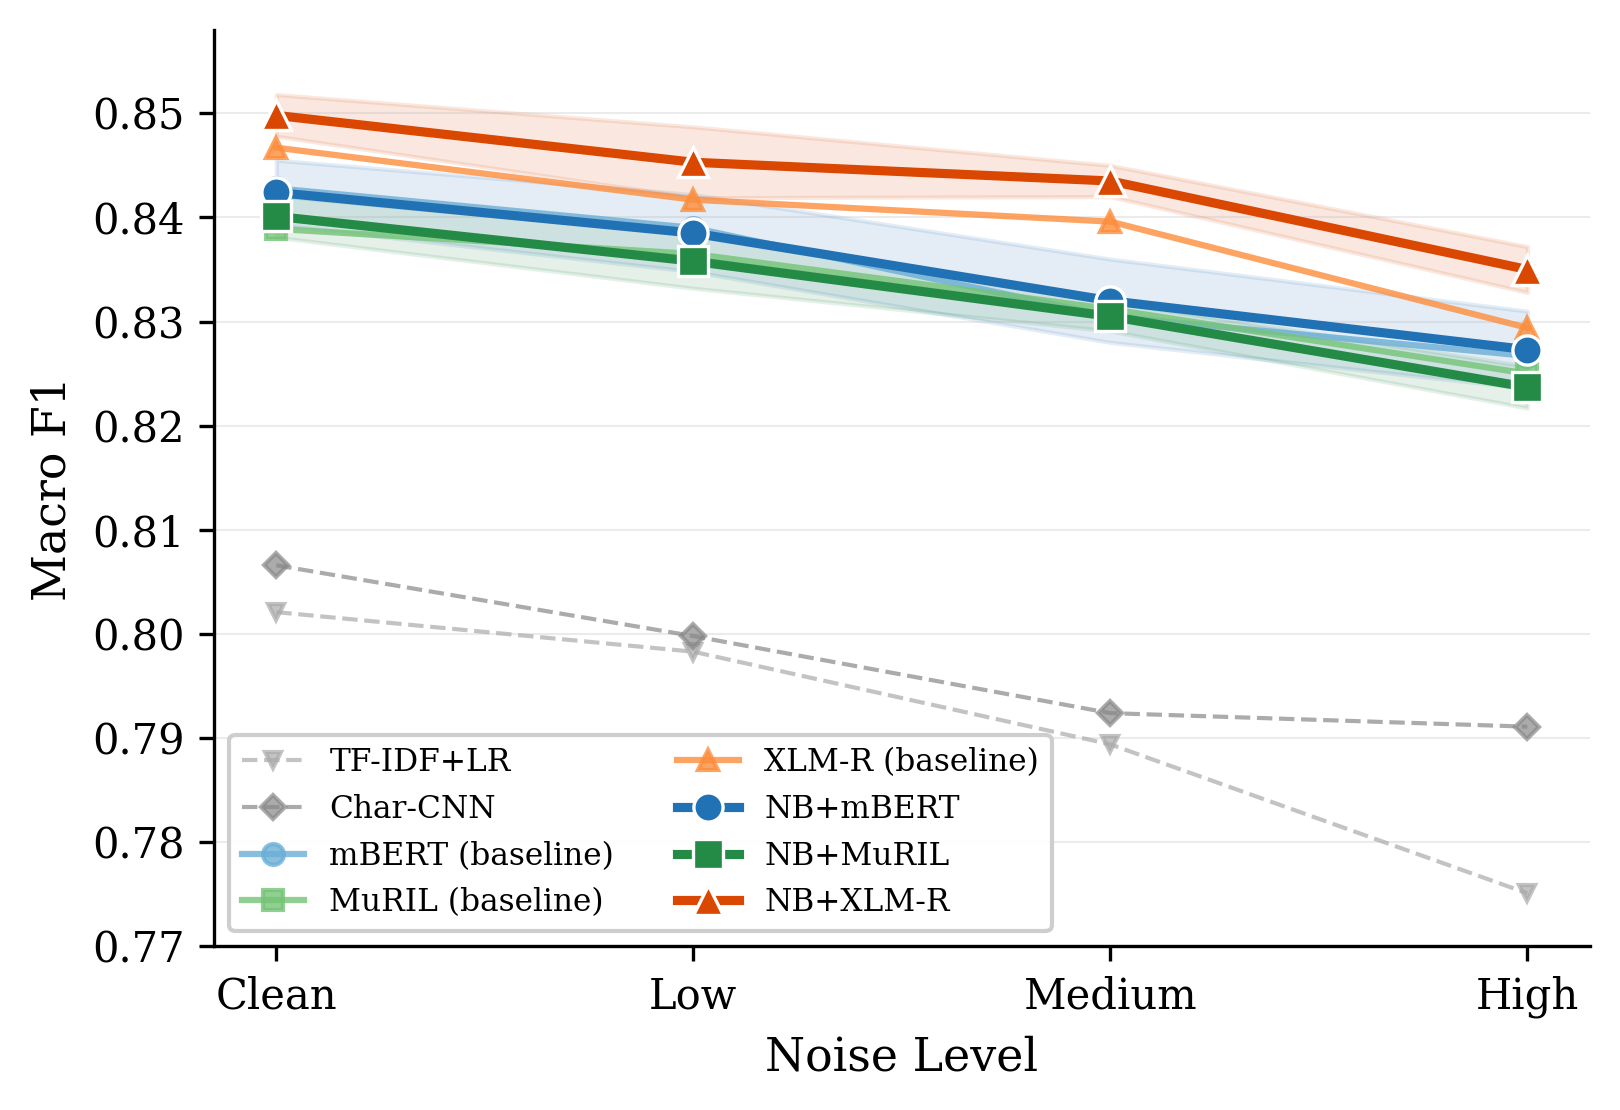
\includegraphics[width=\columnwidth]{fig_degradation.png}
\caption{Performance degradation under increasing ASR noise. XLM-R + NoiseBridge (dark orange, top curve) maintains the flattest degradation, with the gap over the XLM-R baseline widening at higher noise. Shaded bands show $\pm$1 std over 3 seeds.}
\label{fig:degradation}
\end{figure}

\textbf{Finding 1: Transformer encoders are already robust.} All three transformer baselines degrade by only 1.0--1.7 F1 points from clean to high noise, substantially less than lexical baselines (TF-IDF+LR: $-2.70$). This suggests contextual representations absorb character-level noise effectively.

\textbf{Finding 2: NoiseBridge helps XLM-R consistently.} XLM-R + NoiseBridge improves over the XLM-R baseline on all four conditions ($\Delta_\text{avg} = +0.41$ F1), with the largest gain on high noise ($+0.56$). For mBERT and MuRIL, deltas are within seed variance ($\Delta_\text{avg} \approx 0$).

\textbf{Finding 3: Improvement scales with noise severity.} For XLM-R, the delta grows monotonically: $+0.31$ (clean) $\to$ $+0.36$ (low) $\to$ $+0.39$ (medium) $\to$ $+0.56$ (high), confirming that PWNIC provides increasing benefit as noise worsens.

\textbf{Why XLM-R benefits while others do not.} We hypothesize that XLM-R's SentencePiece tokenizer preserves more phonetic structure than mBERT's and MuRIL's WordPiece. SentencePiece operates on raw Unicode codepoints without language-specific normalization, while WordPiece applies case folding and accent stripping that can collapse phonetic distinctions relevant to Hinglish.

% ============================================================================
\section{Analysis}
\label{sec:analysis}
% ============================================================================

\subsection{Component Ablation}

Table~\ref{tab:components} and Fig.~\ref{fig:components} show the contribution of each NoiseBridge component on XLM-R (seed 42, average F1 across all four test conditions).

\begin{table}[!t]
\caption{Additive Component Analysis (XLM-R, Avg F1)}
\label{tab:components}
\centering
\small
\begin{tabular}{lccc}
\toprule
\textbf{Configuration} & $\alpha$ & $\gamma$ & \textbf{Avg F1} \\
\midrule
XLM-R baseline (CE only) & -- & -- & 0.8394 \\
\quad + Noise-aware gate  & 0   & 0   & 0.8339 \\
\quad\quad + PWNIC         & 0.15& 0   & 0.8401 \\
\quad\quad\quad + Aux      & 0.15& 0.2 & \textbf{0.8434} \\
\midrule
Full NB v1 (+ GRL)        & 0.15& 0.1 & 0.8237 \\
\bottomrule
\end{tabular}
\end{table}

\begin{figure}[!t]
\centering
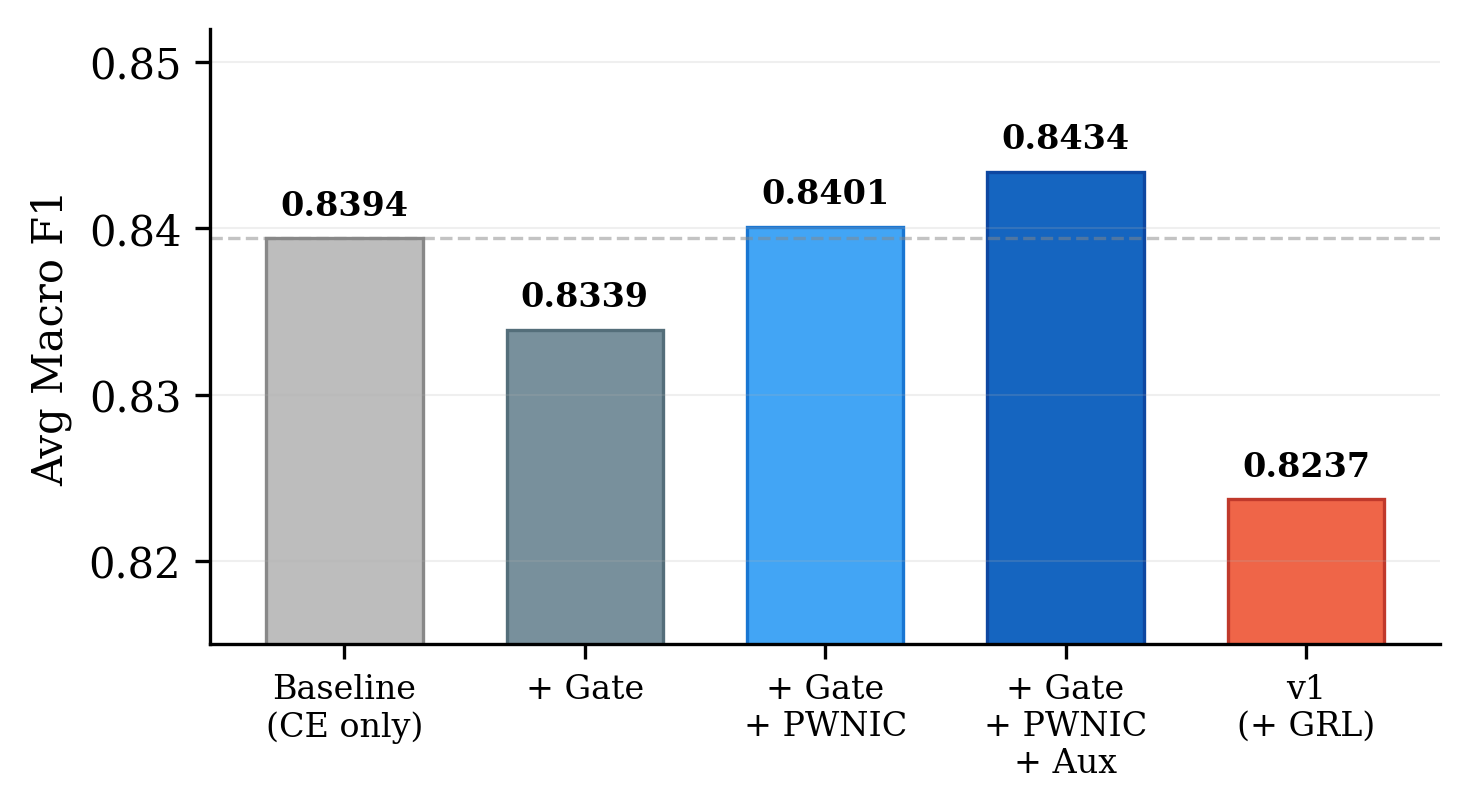
\includegraphics[width=\columnwidth]{fig_components.png}
\caption{Component ablation on XLM-R. The noise-aware gate alone slightly hurts ($-0.55$ from baseline). Adding PWNIC recovers and exceeds baseline ($+0.07$). The auxiliary head provides a further $+0.33$ gain. Adding GRL (v1 design) catastrophically degrades performance ($-1.57$ from baseline).}
\label{fig:components}
\end{figure}

An interesting finding is that the noise-aware gate \textit{alone} slightly hurts performance (0.8339 vs.\ 0.8394 baseline). This suggests that without the contrastive signal from PWNIC to guide it, the gate learns to suppress tokens indiscriminately. PWNIC provides the critical training signal ($+0.62$ over gate-only), and the auxiliary head adds a meaningful further boost ($+0.33$).

\subsection{Adversarial Gradient Reversal Ablation}
\label{sec:ablation}

An earlier version of NoiseBridge (v1) included a gradient reversal layer (GRL)~\cite{ganin2016domain} for adversarial noise disentanglement. Table~\ref{tab:ablation} and Fig.~\ref{fig:ablation} present this as a negative result.

\begin{table}[!t]
\caption{v1 (with GRL) vs.\ v2 (without GRL) vs.\ Baseline}
\label{tab:ablation}
\centering
\small
\begin{tabular}{l@{\hskip 6pt}cccc}
\toprule
\textbf{Model} & \textbf{C} & \textbf{L} & \textbf{M} & \textbf{H} \\
\midrule
\multicolumn{5}{l}{\textit{XLM-R}} \\
Baseline       & .847 & .842 & .840 & .829 \\
NB v1 (w/ GRL) & .844 & .840 & .834 & \textcolor{red}{\textbf{.777}} \\
NB v2 (no GRL) & \textbf{.850} & \textbf{.845} & \textbf{.844} & \textbf{.835} \\
\midrule
\multicolumn{5}{l}{\textit{MuRIL}} \\
Baseline       & .839 & .837 & .831 & .825 \\
NB v1 (w/ GRL) & .832 & .834 & \textcolor{red}{\textbf{.786}} & .815 \\
NB v2 (no GRL) & \textbf{.840} & \textbf{.836} & \textbf{.830} & \textbf{.824} \\
\midrule
\multicolumn{5}{l}{\textit{mBERT}} \\
Baseline       & .843 & .839 & .831 & .827 \\
NB v1 (w/ GRL) & .832 & .830 & .822 & .818 \\
NB v2 (no GRL) & \textbf{.842} & \textbf{.839} & \textbf{.832} & \textbf{.827} \\
\bottomrule
\end{tabular}
\end{table}

\begin{figure}[!t]
\centering
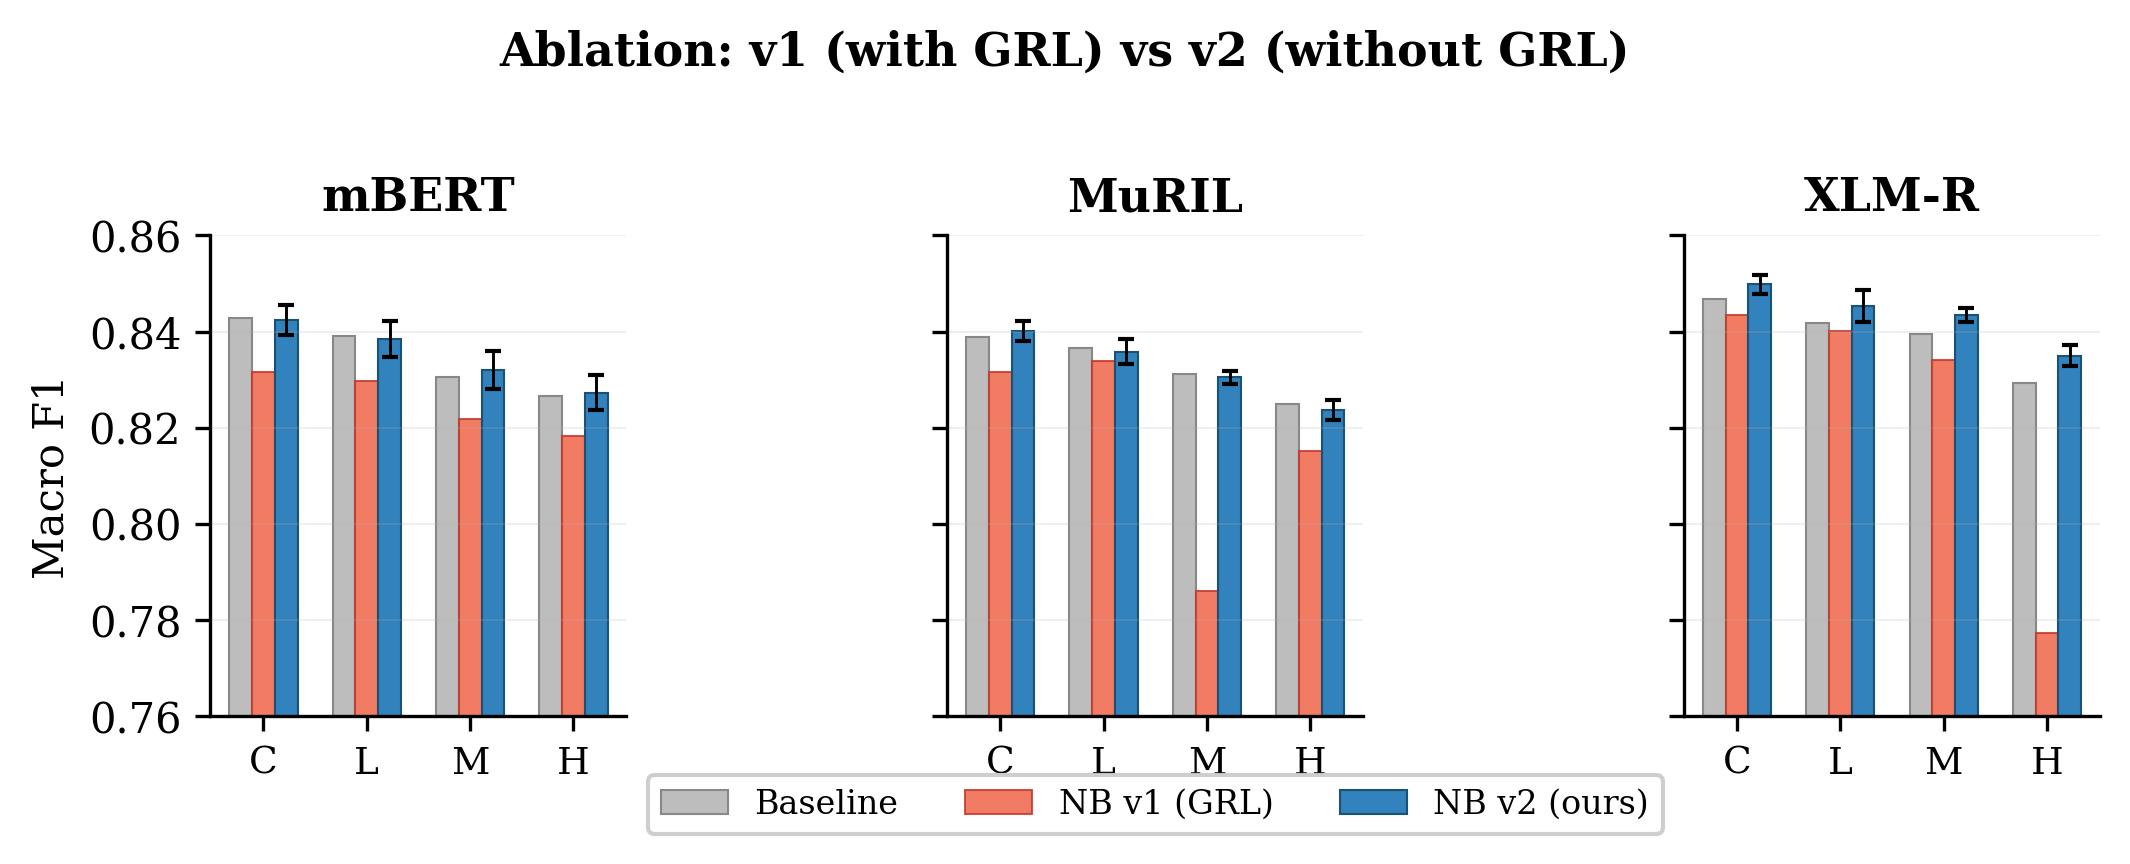
\includegraphics[width=\columnwidth]{fig_ablation.png}
\caption{Ablation across three encoders. Red bars show v1 (GRL) catastrophic failures: XLM-R high ($0.777$, $-5.2$ pts from baseline) and MuRIL medium ($0.786$, $-4.5$ pts). Blue bars show v2 recovery.}
\label{fig:ablation}
\end{figure}

The v1 architecture added a GRL and adversarial noise predictor:
\begin{equation}
\mathcal{L}_{\text{v1}} = \mathcal{L}_\text{CE} + \alpha \mathcal{L}_{\text{PWNIC}} + \beta \mathcal{L}_\text{adv}^{\text{GRL}} + \gamma \mathcal{L}_\text{aux}
\end{equation}
where the GRL reverses gradients from $\mathcal{L}_\text{adv}$ to the encoder.

\textbf{Failure Mode 1: Degenerate Targets.} When training on a single noise level, all noise labels are identical ($y_i^\text{noise} = c$ $\forall i$). The adversarial predictor trivially achieves zero loss; the GRL then pushes the encoder toward uniform representations, destroying the classification signal. This explains the XLM-R high collapse (0.777) and MuRIL medium collapse (0.786).

\textbf{Failure Mode 2: Contradictory Gradients.} The adversarial head ($\beta = 0.3$, with GRL) and auxiliary head ($\gamma = 0.1$, without GRL) operate on the same $\mathbf{z}^n$ with opposite objectives. With $\beta > \gamma$, the adversarial gradient dominates and the auxiliary head becomes noise.

These findings led us to remove the GRL entirely in v2, keeping only the auxiliary predictor with auto-disable for single-noise-level conditions.

\subsection{Phonetic Weight Analysis}

Fig.~\ref{fig:phi} shows the distribution of phonetic dissimilarity weights $\phi$ ((\ref{eq:phi})) across noise levels. The monotonic increase in mean $\phi$ (low: 0.025, medium: 0.039, high: 0.056) confirms that the weighting correctly assigns stronger contrastive pressure to more distorted examples.

\begin{figure}[!t]
\centering
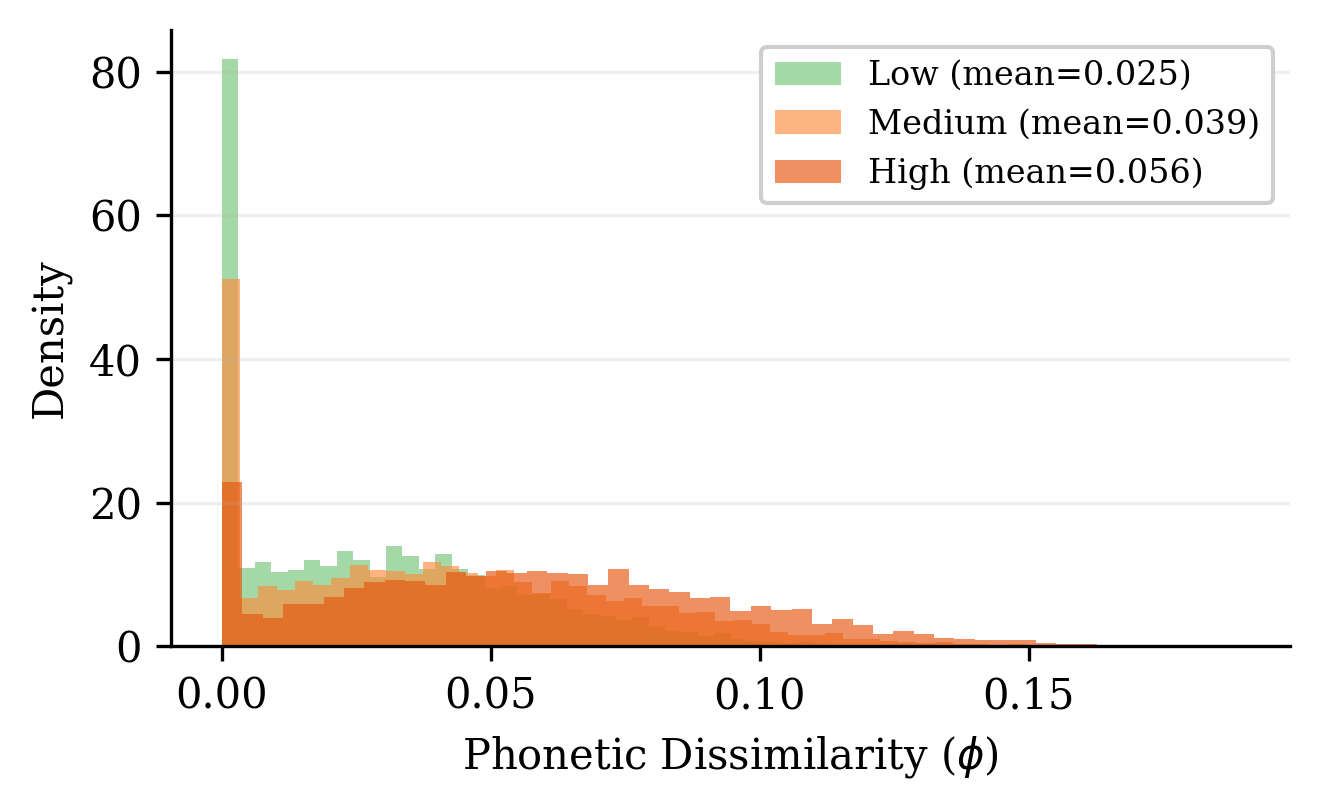
\includegraphics[width=\columnwidth]{fig_phi_dist.png}
\caption{Distribution of PWNIC weights $\phi$ by noise level. Higher noise produces higher $\phi$, triggering stronger contrastive alignment.}
\label{fig:phi}
\end{figure}

\subsection{Error Analysis}

We inspect 50 examples where XLM-R + NoiseBridge differs from the baseline on the high-noise test set. Three patterns emerge: (1)~\textit{Noisy Hinglish slurs} (24/50): partially corrupted slurs (e.g., ``madarchod'' $\to$ ``madrachd'') defeat the baseline but are correctly classified by NoiseBridge, suggesting PWNIC maps corrupted representations near their clean counterparts. (2)~\textit{Word boundary errors} (14/50): ASR-style word splits (``chutiya'' $\to$ ``chu ti ya'') break tokens into individually non-hateful subwords; the gate appears to down-weight fragments. (3)~\textit{English text unaffected} (12/50): minor noise on English text produces near-boundary differences.

% ============================================================================
\section{Discussion}
\label{sec:discussion}
% ============================================================================

\textbf{When Does NoiseBridge Help?} PWNIC is most effective when the encoder's tokenization preserves phonetic structure. XLM-R's SentencePiece retains sub-character patterns responsive to contrastive alignment; mBERT's and MuRIL's WordPiece normalizes these away. This suggests noise-robustness interventions should be co-designed with the tokenizer.

\textbf{Against Adversarial Disentanglement.} We tested $\beta \in \{0.1, 0.3, 0.5\}$ and $\lambda_\text{max} \in \{0.5, 1.0\}$; all underperformed the no-GRL baseline. The root cause---degenerate targets when noise level is constant---is structural, not tunable. This contrasts with DANN's success in domain adaptation~\cite{ganin2016domain} where domains are always distinct.

\textbf{Byte-Level Encoders.} Preliminary experiments with ByT5-small~\cite{xue2022byt5} achieved validation F1 of 0.831 after one epoch (FP32 required; T5 overflows under FP16 on Tesla T4 hardware). While comparable to MuRIL, training time (${\sim}9$ hours/epoch) prevented full evaluation. The interaction between byte-level phonetic structure and PWNIC remains a promising direction for future work.

\textbf{Limitations.} Our noise is synthetic (character-level perturbations), not from real ASR transcripts. The benchmark is English-heavy (80.7\% in test). Gains are modest ($+0.41$ avg F1), suggesting a low noise-robustness ceiling for current multilingual encoders.

% ============================================================================
\section{Conclusion}
% ============================================================================

We presented HindiMix-Noisy, the first ASR-noise benchmark for Hindi-English code-mixed hate speech, and NoiseBridge, a phonetic-weighted contrastive framework. Key findings: (1)~multilingual encoders degrade only 1--2 F1 under high noise; (2)~PWNIC provides consistent gains with XLM-R ($+0.41$ avg, $+0.56$ high noise); (3)~adversarial gradient reversal fails catastrophically in this setting. The benchmark, code, and models are publicly available.\footnote{\url{https://github.com/PLACEHOLDER/noisebridge}}

\begin{thebibliography}{00}
\bibitem{barman2014code} U.~Barman, A.~Das, J.~Wagner, and J.~Foster, ``Code mixing: A challenge for language identification in the language of social media,'' in \textit{Proc. First Workshop on Computational Approaches to Code Switching}, 2014.
\bibitem{basile2019semeval} V.~Basile et al., ``SemEval-2019 Task 5: Multilingual detection of hate speech against immigrants and women in Twitter,'' in \textit{Proc. SemEval}, 2019.
\bibitem{belinkov2018synthetic} Y.~Belinkov and Y.~Bisk, ``Synthetic and natural noise both break neural machine translation,'' in \textit{Proc. ICLR}, 2018.
\bibitem{bohra2018dataset} A.~Bohra, D.~Vijay, V.~Singh, S.~S.~Akhtar, and M.~Shrivastava, ``A dataset of Hindi-English code-mixed social media text for hate speech detection,'' in \textit{Proc. PEOPLES}, 2018.
\bibitem{caselli2020hatebert} T.~Caselli, V.~Basile, J.~Mitrovi{\'c}, and M.~Granitzer, ``HateBERT: Retraining BERT for abusive language detection in English,'' in \textit{Proc. WOAH}, 2020.
\bibitem{chen2020simclr} T.~Chen, S.~Kornblith, M.~Norouzi, and G.~Hinton, ``A simple framework for contrastive learning of visual representations,'' in \textit{Proc. ICML}, 2020.
\bibitem{conneau2020xlmr} A.~Conneau et al., ``Unsupervised cross-lingual representation learning at scale,'' in \textit{Proc. ACL}, 2020.
\bibitem{davidson2017automated} T.~Davidson, D.~Warmsley, M.~Macy, and I.~Weber, ``Automated hate speech detection and the problem of offensive language,'' in \textit{Proc. ICWSM}, 2017.
\bibitem{devlin2019bert} J.~Devlin, M.-W.~Chang, K.~Lee, and K.~Toutanova, ``BERT: Pre-training of deep bidirectional transformers for language understanding,'' in \textit{Proc. NAACL}, 2019.
\bibitem{eger2019text} S.~Eger et al., ``Text processing like humans do: Visually attacking and shielding NLP systems,'' in \textit{Proc. NAACL}, 2019.
\bibitem{ganin2016domain} Y.~Ganin et al., ``Domain-adversarial training of neural networks,'' \textit{JMLR}, vol.~17, no.~1, pp.~2096--2030, 2016.
\bibitem{gao2021simcse} T.~Gao, X.~Yao, and D.~Chen, ``SimCSE: Simple contrastive learning of sentence embeddings,'' in \textit{Proc. EMNLP}, 2021.
\bibitem{khanuja2020gluecos} S.~Khanuja et al., ``GLUECoS: An evaluation benchmark for code-switched NLP,'' in \textit{Proc. ACL}, 2020.
\bibitem{khanuja2021muril} S.~Khanuja et al., ``MuRIL: Multilingual representations for Indian languages,'' \textit{arXiv:2103.10730}, 2021.
\bibitem{khosla2020supervised} P.~Khosla et al., ``Supervised contrastive learning,'' in \textit{Proc. NeurIPS}, 2020.
\bibitem{loshchilov2019decoupled} I.~Loshchilov and F.~Hutter, ``Decoupled weight decay regularization,'' in \textit{Proc. ICLR}, 2019.
\bibitem{mandl2021hasoc} T.~Mandl et al., ``Overview of the HASOC subtrack at FIRE 2021,'' in \textit{Proc. FIRE}, 2021.
\bibitem{mathew2021hatexplain} B.~Mathew et al., ``HateXplain: A benchmark dataset for explainable hate speech detection,'' in \textit{Proc. AAAI}, 2021.
\bibitem{mozafari2020bert} M.~Mozafari, R.~Farahbakhsh, and N.~Crespi, ``A BERT-based transfer learning approach for hate speech detection,'' in \textit{Proc. COMPLEX NETWORKS}, 2020.
\bibitem{oord2018representation} A.~van~den~Oord, Y.~Li, and O.~Vinyals, ``Representation learning with contrastive predictive coding,'' \textit{arXiv:1807.03748}, 2018.
\bibitem{piktus2019misspelling} A.~Piktus et al., ``Misspelling oblivious word embeddings,'' in \textit{Proc. NAACL}, 2019.
\bibitem{pratapa2018language} A.~Pratapa et al., ``Language modeling for code-mixing,'' in \textit{Proc. ACL}, 2018.
\bibitem{shah2020learning} P.~Shah, H.~S.~Chadha, A.~Gupta, and A.~Bharadwaj, ``Learning to recognize speech in Hindi-English code-mixed environments,'' \textit{arXiv:2011.12610}, 2020.
\bibitem{winkler1990string} W.~E.~Winkler, ``String comparator metrics and enhanced decision rules in the Fellegi-Sunter model,'' \textit{Proc. Survey Research Methods, ASA}, 1990.
\bibitem{xue2022byt5} L.~Xue et al., ``ByT5: Towards a token-free future with pre-trained byte-to-byte models,'' \textit{TACL}, vol.~10, pp.~291--306, 2022.
\bibitem{zampieri2019predicting} M.~Zampieri et al., ``Predicting the type and target of offensive posts in social media,'' in \textit{Proc. NAACL}, 2019.
\bibitem{zhang2015character} X.~Zhang, J.~Zhao, and Y.~LeCun, ``Character-level convolutional networks for text classification,'' in \textit{Proc. NeurIPS}, 2015.
\end{thebibliography}

\end{document}
